% v4 Results part D: estimating the state from the wall (register R14-R21).
% Written LAST per the spec; carries the resolved F20-B branch (NIS
% refutation with mechanism + the coverage-band two-stage addendum) and the
% resolved FK16-B branch (seed fragility). The excluded test-selected
% variant appears ONLY in the calibration disclosure appendix (D3).

\subsubsection{The estimator ladder, its calibration and its deployment envelope}
\label{sec:res_da}

\rb{K}{S4D-01}{Physical units reorganise the phase story and expose the relaxation $R^2$ as a variance artefact. Decision D252 in one paragraph.}Physical units reorganise the phase story. Read in $R^2$ the relaxation
phase looks like a failure; read in lift units it is the best phase the estimator
has, because the relaxation variance is small and the ratio, not the error,
collapses (figure~\ref{fig:tracking}, which carries the per-phase errors).
Assimilation is decisive at impact: the filter cuts the open-loop drift about
five-fold, to \DapRexImpRmse{} in lift units, with the median peak error at
\DapRexPeakErr{} per cent of the true peak and peak timing within one
frame. Relative accuracy is approximately scale-invariant across the training
envelope, near $12$ to $14$ per cent for the
forecast-derived filter at all but the $|G| = 1$ stratum, which sits somewhat
higher, while the linear filter is non-uniform
(figure~\ref{fig:relerr}); the absolute error grows with the peak it
tracks, which is what a scale-invariant estimator must do.\re

\rb{K}{S4D-02}{The estimator ladder with the static inverse on top, the qualifier that scopes the entire estimation result. The abstract depends on this paragraph.}The estimator ladder orders the suite at impact
(appendix~\ref{app:calibration}, figure~\ref{fig:calibration}), and its top rung is unexpected:
the \StaticInv, no dynamics at all, matches the best
\TestSplit{} impact medians on the ladder (\DapEobsImpRTwo;
figure~\ref{fig:calibration}a). The filters' case does not rest
on the in-distribution median. It rests on the tails, where the
\StaticInv{} posts a large-error encounter, its impact-phase
$R^2$ falling below $-1$; on the
extrapolation boundary, where the \TwoStageKF{} reaches
\PoneTwoStageCovImpactC{} median $R^2$ on the $|G| = 4$ \BoundarySplit{}
encounters with no large-error case and a positive relaxation
(\PoneTwoStageCovRelaxC); and on state tracking beyond the single read-out
the inverse regresses. The linear filter with encoded observations adds
the robustness column: zero consistency failures under the fixed criterion of
\S\ref{sec:methods_lae} and graceful degradation as the assimilation rate
drops, where the base filter collapses already at
every-second-frame updates (supplementary material).\re

\rb{A}{S4D-03}{The full calibration narrative, including the excluded test-selected variant, told at length in the body. Appendix C already exists for exactly this audit trail; the body needs the one-sentence outcome.}Calibrating the forecast-derived noise did not go the way the calibration
hypothesis expected, and the failure is informative. On the held-out
training encounters the pooled impact-phase innovation statistic sits
below one at every band scale in the grid fixed in advance (\PoneNisAtCStar{}
at the selected edge $c^{*} = \PoneNisCStar$) while the same split's
tracking improves monotonically with the band
(figure~\ref{fig:calibration}): innovation consistency and tracking
optimality point in opposite directions, so the frozen NIS-selected run, the
single-stage forecast-noise filter at the NIS-selected band $c^{*}$, closes at
\PoneFrozenRexImpact{} at impact on the \TestSplit{} set, below the
production two-stage rung, and the
consistency route to a larger band is not supported by the held-out
training encounters. The mechanism is model
error, not miscalibration: inflating the state-dependent noise compensates
the forecast median's contraction, buying gain at the price of
consistency, and the test-selected variant excluded by the freeze rule is
disclosed, with its number, only in appendix~\ref{app:calibration}. The
five-seed member-noise mean of the \FnoiseKF{} at this band is
\PoneRexEnkfImpact{} at impact. The legitimate gain comes from structure instead of noise: the
\TwoStageKF{} of \S\ref{sec:methods_rexenkf}, at the production coverage
band (a single validation-calibrated noise scale, no test-set tuning),
reaches \PoneTwoStageCovImpact{} at impact on
the \TestSplit{} set (root-mean-square error \PoneTwoStageCovRmse) and carries the
\BoundarySplit{} set as above, the best filter in the ladder among those selected without reference to
the test set.\re

\rb{K}{S4D-04}{The smoother result and the deployment rule it changes. Short, concrete and cited in appendix B guidance.}When a quarter-convective-time latency is acceptable, the smoother
changes the deployment rule. The fixed-lag recursion of
the fixed-lag smoother of appendix~\ref{app:rts} on the linear stack cuts the impact error to
\SmRtsImpRmse{} from the filter's \SmKfImpRmse{} and leaves the relaxation
essentially unchanged (\SmRtsRelRmse{} against
\SmKfRelRmse), a full-interval reanalysis at lag five;
the ensemble smoother on the \FnoiseKF{} degrades it
(supplementary material). Online estimation therefore takes the
nonlinear filter and a $0.25\,t/c$ latency budget takes the closed-form
linear smoother.\re

\rb{K}{S4D-05}{The per-family end-to-end comparison, which is the fair version of the estimator claim. Also the sensor-budget and noise-robustness separation.}What the training objective confers survives to the assimilation stage, and
per-family end-to-end evaluation makes the comparison fair: each family senses at its
own sensors, encodes its own observations, forecasts with its own operator
and decodes through its own decoder. The \PredState{}
cuts the reconstructive anchor's assimilated load error by more than a third
at impact and by more than half in relaxation
(impact \OwnClwImpRmse{} against \OwnAeLwImpRmse, relaxation
\OwnClwRelRmse{} against \OwnAeLwRelRmse; the \LiftState{} between at
\OwnClnImpRmse), while decoded-field fidelity is family-insensitive
(figure~\ref{fig:ownstack}a). The sensor axis separates the families
further: the predictive state exploits every added sensor monotonically
where the reconstructive one saturates at $K = 8$, and it degrades more
slowly with sensor noise, still beating the clean reconstructive stack at
twenty per cent noise (figure~\ref{fig:ownstack}b,c). Streaming
multi-encounter assimilation under a deployment-realism protocol, and a
filter on the four-dimensional lift-critical state of
\S\ref{sec:res_dimension}, are reported in appendix~\ref{app:sensing}.\re

\rb{K}{S4D-06}{The dimension-by-family grid and the reconstructive seed fragility, with the observation-side mechanism verified. This is the deployment-robustness argument of the paper.}The closing study runs the whole design axis through one identical
per-family end-to-end protocol: three families at four dimensions
(figure~\ref{fig:dimsgrid}). The predictive family is uniform, impact
error between \GridJepDThirtyTwoRmse{} and \GridJepDEightRmse{} across
$d \in \{4, 8, 16, 32\}$ with peak errors of ten to fifteen per cent
everywhere; even its $d = 4$ cell (\GridJepDFourRmse) beats the linear
floor's best (\GridPodDThirtyTwoRmse{} at $d = 32$). The linear basis is
stable and a step worse everywhere. The reconstructive baseline is
non-monotonic in dimension and irreproducible across seeds: it fails
outright at $d = 4$ and $d = 32$ (\GridFkDFourRmse{} and \GridFkDThirtyTwoRmse, peak errors
above one hundred per cent, assimilation at $d = 32$ making the open loop
worse), and its $d = 16$ cell, the best single cell in the
grid at \GridFkDSixteenRmse{}, does not survive seed replication: across
three encoder seeds the same cell spans \PoneFkSixteenImpactRmse{} impact
error on average with individual seeds at $0.18$, $0.65$ and $5.9$, the
worst of them failing exactly as the neighbouring dimensions do. The
mechanism is verified and lives on the observation side: linear probes on
the true reconstructive latents are healthy at every dimension and every
seed, while the pressure-to-latent map fails to recover the lift-carrying
directions, insensitive to its regularisation, under a protocol that
succeeds for the other two families in every cell. Wall-pressure
estimatability of the reconstructive geometry is unpredictable across
both dimension and training seed; the anchored families are uniformly
estimatable, which is the deployment-robustness argument of this paper.\re

\rb{T}{S4D-07}{Two loose ends that restate \S4.6.2's under-dispersion and \S4.5's sensing geometry. Its consistency-failures-removed claim is also the one number in the section with no bound macro.}Two loose ends close the section. The under-dispersion of the base filter
has two regimes, not one: at impact it was calibration, and the
state-dependent noise removes the consistency failures entirely; in
relaxation it is model error, the forecast median's contraction, which no
noise model fixes and the smoother does. And the wake-enstrophy null of
the frozen filter, no family's filter tracks $E_w$, now has its
mechanism: the wall constrains the lift-carrying near-body directions,
the ones the Chang decomposition of \S\ref{sec:methods_chang} weights,
while the wake enstrophy lives in shed structure the sensors reach only
through the delay window, so the null is the sensing geometry, not the
state; the delay-for-sensors trade of \S\ref{sec:res_wall} bounds what
any wall-limited estimator of this flow can see.\re

\begin{figure}
  \centering
  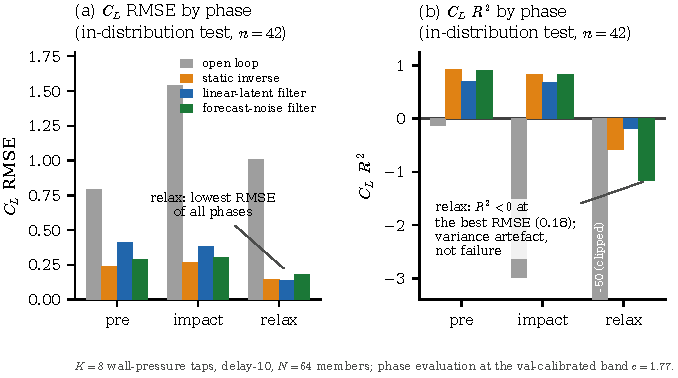
\includegraphics[width=0.82\linewidth]{sections/figures/results/fig_da_tracking_v4.pdf}
  \caption{\rb{K}{S4D-C1}{The phase-resolved tracking figure with the production band stated. Self-contained.}Phase-resolved lift tracking with the \FnoiseKF{} at the production
  coverage band on the \TestSplit{} set
  ($n = 42$
  encounters, $K = 8$ sensors, delay $10$, $N = 64$ members, every-frame pressure).
  Lift error per phase in physical units (a) and in $R^2$ (b) at the
  val-calibrated band: the relaxation $R^2$ collapse is a variance artefact, the
  physical error the honest phase metric. The estimator ladder, its noise
  calibration and the fixed-lag smoother are in
  appendix~\ref{app:calibration} (figure~\ref{fig:calibration}).\re}
  \label{fig:tracking}
\end{figure}




\begin{figure}
  \centering
  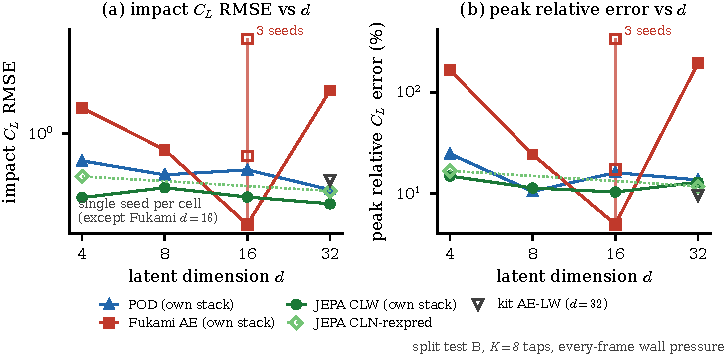
\includegraphics[width=\linewidth]{sections/figures/results/fig_da_dims_grid_v4.pdf}
  \caption{\rb{K}{S4D-C2}{The dimension grid, with the single-seed disclosure per cell. Self-contained.}The assimilation-versus-dimension grid (\TestSplit{} set, per-family end-to-end stacks,
  $K = 8$, every-frame pressure; single seed per cell except the
  reconstructive $d = 16$ cell, which carries three): impact error and
  relative peak error against dimension for the three families. The
  predictive family is uniform, the linear basis stable, the
  reconstructive baseline non-monotonic in dimension and irreproducible
  across seeds.\re}
  \label{fig:dimsgrid}
\end{figure}
